% PyTorch Conference North America 2026 poster
% Official max size: 24in x 34in (A1), one-sided, CMYK, <100MB
% Build:  cd tex/poster && tectonic poster.tex
%
% Numbers on this board are the held-out Slurm split and the live
% VGAC model card. Do not restore AUROC 0.985 / ECE 0.006.

\documentclass[12pt]{article}

\usepackage[paperwidth=24in,paperheight=34in,margin=0.38in]{geometry}
\usepackage{fontspec}
\setmainfont{Helvetica Neue}
\setsansfont{Helvetica Neue}
\renewcommand{\familydefault}{\sfdefault}

\usepackage[cmyk]{xcolor}
\usepackage{graphicx}
\usepackage{tikz}
\usetikzlibrary{arrows.meta,positioning}
\usepackage{enumitem}
\usepackage{qrcode}
\usepackage{microtype}
\usepackage[hidelinks]{hyperref}

\pagestyle{empty}
\setlength{\parindent}{0pt}
\setlength{\parskip}{0pt}
\setlist[itemize]{leftmargin=1.1em,itemsep=0.16em,topsep=0.12em,parsep=0pt,partopsep=0pt}

\definecolor{navy}{cmyk}{0.92,0.72,0.38,0.48}
\definecolor{navy2}{cmyk}{0.78,0.55,0.30,0.28}
\definecolor{pytorch}{cmyk}{0.00,0.82,0.88,0.07}
\definecolor{sand}{cmyk}{0.04,0.06,0.12,0.02}
\definecolor{warn}{cmyk}{0.00,0.28,0.85,0.00}
\definecolor{ok}{cmyk}{0.72,0.08,0.68,0.18}
\definecolor{ink}{cmyk}{0.00,0.00,0.00,0.88}
\definecolor{muted}{cmyk}{0.08,0.06,0.06,0.48}
\definecolor{suggest}{cmyk}{0.55,0.18,0.00,0.08}
\definecolor{cardline}{cmyk}{0.12,0.08,0.08,0.08}

\newcommand{\figpath}{../../figures}
\newlength{\colw}
\setlength{\colw}{0.318\textwidth}
\newcommand{\gutterh}{\hspace{0.023\textwidth}}

\newcommand{\kicker}[1]{%
  {\fontsize{12.5}{15}\selectfont\bfseries\color{pytorch}\MakeUppercase{#1}\par}\vspace{0.06in}}
\newcommand{\sectionhead}[1]{%
  {\fontsize{24}{28}\selectfont\bfseries\color{navy}#1\par}\vspace{0.14in}}
\newcommand{\body}{\fontsize{16.5}{21}\selectfont\color{ink}}
\newcommand{\smallbody}{\fontsize{15}{19}\selectfont\color{ink}}
\newcommand{\captiontext}{\fontsize{13}{16.5}\selectfont\color{muted}}

\begin{document}
\pagecolor{white}
\color{ink}

% ── Header ──────────────────────────────────────────────────────────
\begin{tikzpicture}[remember picture,overlay]
  \fill[navy] (current page.north west) rectangle ([yshift=-2.62in]current page.north east);
  \fill[pytorch] (current page.north west) ++(0,-2.62in) rectangle ([yshift=-2.74in]current page.north east);
\end{tikzpicture}

\vspace*{-0.06in}
\begin{minipage}[t]{0.79\textwidth}
  {\fontsize{13}{16}\selectfont\color{sand}\bfseries
    PYTORCH CONFERENCE NORTH AMERICA 2026 \quad$\cdot$\quad
    COMMUNITY EXPO \quad$\cdot$\quad TUE 20 OCT 5:45--7:15 PM}\\[0.20in]
  {\fontsize{44}{48}\selectfont\bfseries\color{white}What Should SRE Watch?}\\[0.10in]
  {\fontsize{22}{26}\selectfont\color{sand}Calibration-Gated Decisions and the Missing Golden Signals for GPU Clusters}\\[0.20in]
  {\fontsize{16.5}{20}\selectfont\color{white}
    Andrew Espira \quad$\cdot$\quad Saint Peter's University \quad$\cdot$\quad
    \href{https://demo.vgac.cloud/}{\color{white}demo.vgac.cloud}}
\end{minipage}%
\hfill
\begin{minipage}[t]{1.9in}
  \vspace{0.02in}
  
\begin{tikzpicture}
    \fill[white] (0,0) rectangle (1.88in,1.88in);
    \node at (0.94in,0.94in) {\qrcode[height=1.58in]{https://demo.vgac.cloud/}};
  \end{tikzpicture}\\[-0.02in]
  {\centering\fontsize{11}{13}\selectfont\color{sand}scan for live demo\par}
\end{minipage}

\vspace{0.62in}

% ── Takeaway (no \% inside; it comments out tikz node text) ─────────
\noindent
\colorbox{pytorch}{%
  \parbox{\dimexpr\textwidth-2\fboxsep-2\fboxrule}{%
    \vspace{0.10in}
    {\fontsize{21}{26}\selectfont\bfseries\color{white}
    Queue wait is the user-visible latency on a shared GPU cluster.
    GPU utilization does not see it.
    We measure Queue-of-Work Reliability (QWR) --- a calibrated
    $P(\mathrm{wait}>\mathrm{SLO})$ --- and gate actions on its ECE.
    The live production model is at ECE 0.068: \emph{warn}, not admit.}
    \vspace{0.10in}
  }%
}

\vspace{0.32in}

% ── Three columns ───────────────────────────────────────────────────
\begin{minipage}[t]{\colw}
\kicker{The four travel poorly}
\sectionhead{Classical golden signals}

{\body
Google SRE's four --- latency, traffic, errors, saturation --- assume a
stateless request/response service. On shared GPU clusters each category
needs a different operational definition.
}

\vspace{0.16in}
{\body
{\bfseries\color{navy}Latency} has token, batch, epoch, \emph{and queue}
meanings. Submit-to-start often dominates. HTTP p99 never sees it.

\vspace{0.12in}
{\bfseries\color{navy}Traffic} as QPS is undefined for training.
Tokens/s and active jobs are different loads.

\vspace{0.12in}
{\bfseries\color{navy}Errors} as HTTP 5xx miss silent quality failure
(200 + a bad output) and OOM / throttle restarts.

\vspace{0.12in}
{\bfseries\color{navy}Saturation} as \texttt{nvidia-smi} utilization is
time-busy, not useful compute. Memory-bound kernels, thermal trips, and
NCCL stragglers can all look fully utilized.
}

\vspace{0.18in}
{\captiontext
These are mechanistic failure modes, not $r$-values from this trace.
The Slurm DCGM slice is idle T4 queue-wait (utilization $=0$), so a
util--goodput correlation is undefined.}
\end{minipage}%
\gutterh
\begin{minipage}[t]{\colw}
\kicker{A paging-rotation minimum}
\sectionhead{Five candidate signals}

{\smallbody
\noindent
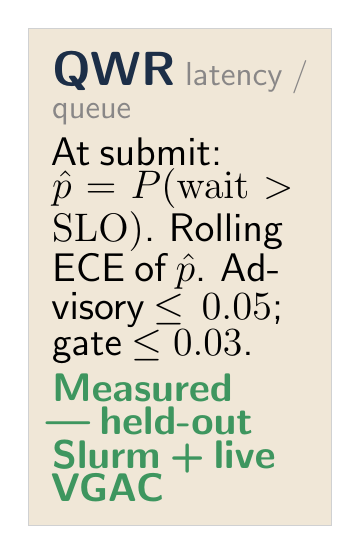
\begin{tikzpicture}
  \node[draw=cardline, fill=sand, inner sep=0.12in, text width=\dimexpr\colw-0.24in\relax, align=left] {
    {\fontsize{17}{20}\selectfont\bfseries\color{navy}QWR}%
    {\fontsize{13}{16}\selectfont\color{muted}  \  latency / queue}\\[0.05in]
    {\fontsize{14.5}{18}\selectfont At submit: $\hat p = P(\mathrm{wait}>\mathrm{SLO})$. Rolling ECE of $\hat p$. Advisory $\le 0.05$; gate $\le 0.03$.}\\[0.04in]
    {\fontsize{14}{17}\selectfont\bfseries\color{ok}Measured --- held-out Slurm + live VGAC}
  };
\end{tikzpicture}\\[0.10in]
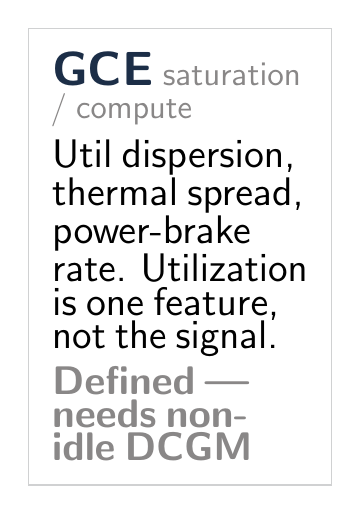
\begin{tikzpicture}
  \node[draw=cardline, fill=white, inner sep=0.12in, text width=\dimexpr\colw-0.24in\relax, align=left] {
    {\fontsize{17}{20}\selectfont\bfseries\color{navy}GCE}%
    {\fontsize{13}{16}\selectfont\color{muted}  \  saturation / compute}\\[0.05in]
    {\fontsize{14.5}{18}\selectfont Util dispersion, thermal spread, power-brake rate. Utilization is one feature, not the signal.}\\[0.04in]
    {\fontsize{14}{17}\selectfont\bfseries\color{muted}Defined --- needs non-idle DCGM}
  };
\end{tikzpicture}\\[0.10in]
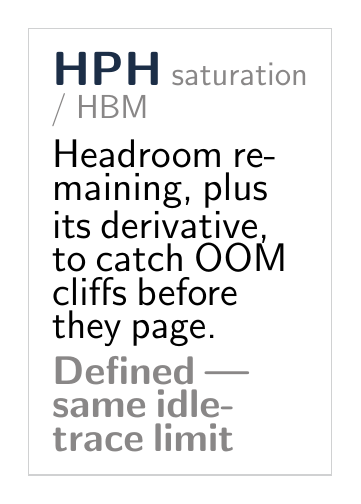
\begin{tikzpicture}
  \node[draw=cardline, fill=white, inner sep=0.12in, text width=\dimexpr\colw-0.24in\relax, align=left] {
    {\fontsize{17}{20}\selectfont\bfseries\color{navy}HPH}%
    {\fontsize{13}{16}\selectfont\color{muted}  \  saturation / HBM}\\[0.05in]
    {\fontsize{14.5}{18}\selectfont Headroom remaining, plus its derivative, to catch OOM cliffs before they page.}\\[0.04in]
    {\fontsize{14}{17}\selectfont\bfseries\color{muted}Defined --- same idle-trace limit}
  };
\end{tikzpicture}\\[0.10in]
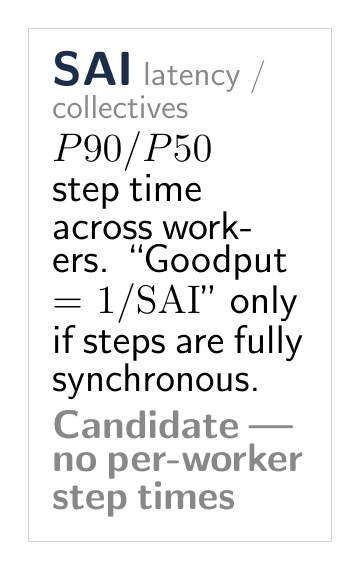
\begin{tikzpicture}
  \node[draw=cardline, fill=white, inner sep=0.12in, text width=\dimexpr\colw-0.24in\relax, align=left] {
    {\fontsize{17}{20}\selectfont\bfseries\color{navy}SAI}%
    {\fontsize{13}{16}\selectfont\color{muted}  \  latency / collectives}\\[0.05in]
    {\fontsize{14.5}{18}\selectfont $P90/P50$ step time across workers. ``Goodput $=1/\mathrm{SAI}$'' only if steps are fully synchronous.}\\[0.04in]
    {\fontsize{14}{17}\selectfont\bfseries\color{muted}Candidate --- no per-worker step times}
  };
\end{tikzpicture}\\[0.10in]
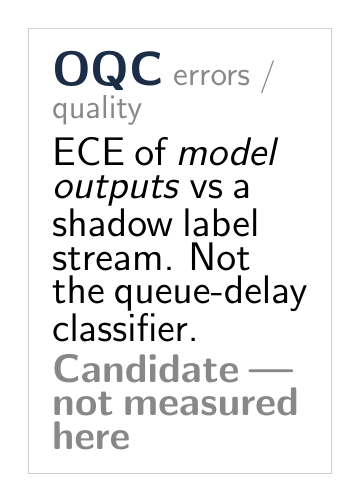
\begin{tikzpicture}
  \node[draw=cardline, fill=white, inner sep=0.12in, text width=\dimexpr\colw-0.24in\relax, align=left] {
    {\fontsize{17}{20}\selectfont\bfseries\color{navy}OQC}%
    {\fontsize{13}{16}\selectfont\color{muted}  \  errors / quality}\\[0.05in]
    {\fontsize{14.5}{18}\selectfont ECE of \emph{model outputs} vs a shadow label stream. Not the queue-delay classifier.}\\[0.04in]
    {\fontsize{14}{17}\selectfont\bfseries\color{muted}Candidate --- not measured here}
  };
\end{tikzpicture}
}
\end{minipage}%
\gutterh
\begin{minipage}[t]{\colw}
\kicker{The title claim}
\sectionhead{The gate currently warns}

{\body
Actions are not ``the model said 70\%.'' They are gated on whether that
70\% is calibrated.
}

\vspace{0.18in}
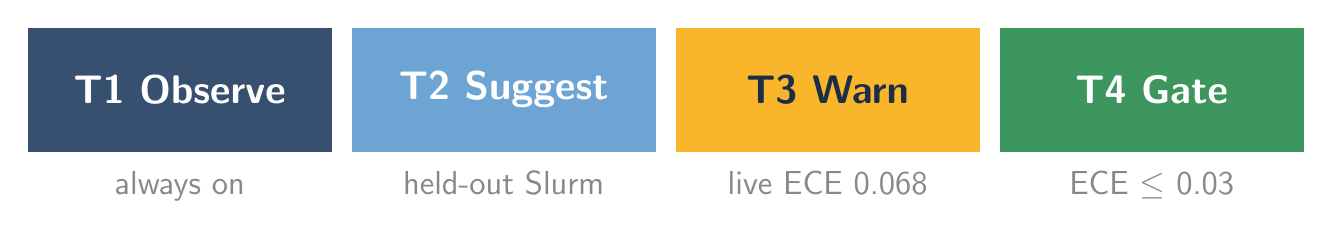
\begin{tikzpicture}[x=1.62in, y=0.78in]
  \foreach \i/\lab/\fill/\fg/\note in {
    0/T1 Observe/navy2/white/always on,
    1/T2 Suggest/suggest/white/held-out Slurm,
    2/T3 Warn/warn/navy/live ECE 0.068,
    3/T4 Gate/ok/white/ECE $\le$ 0.03} {
      \node[draw=none, fill=\fill, text=\fg, font=\bfseries\fontsize{14}{16}\selectfont,
            minimum width=1.52in, minimum height=0.62in, align=center] at (\i,0) {\lab};
      \node[font=\fontsize{11.5}{13.5}\selectfont, text=muted, anchor=north] at (\i,-0.46) {\note};
  }
\end{tikzpicture}

\vspace{0.42in}
{\body
{\bfseries\color{navy}Live VGAC}\\
\texttt{v4.0-richfeatures-lr}\\[0.06in]
ECE \textbf{0.068} \quad AUROC 0.766 \quad $n=5{,}184$\\
Fails 0.05 advisory and 0.03 gate.\\
\textcolor{pytorch}{\bfseries Warn tier --- not T4 Gate.}

\vspace{0.16in}
{\bfseries\color{navy}Held-out Slurm}\\
public \texttt{slurm\_real\_benchmark.json}\\
444 train / 111 test of 555 jobs\\[0.06in]
GB AUROC \textbf{0.863} (CI 0.71--0.96)\\
ECE \textbf{0.056} \quad tier \textbf{suggest}\\
$\sim$8 positives in test \quad 0 true alerts at $p\ge 0.7$

\vspace{0.16in}
{\bfseries\color{navy}Labels are not the same}
\begin{itemize}
  \item EKS long wait: wait $>120$s (near the median).
  \item Slurm long wait: wait $>$ P90 $=133$s ($\sim$10\% base rate).
\end{itemize}
Do not pool AUROC or ECE across those labels.
}

\vspace{0.12in}
{\captiontext
Paper 3 abstract (650 EKS jobs, ECE 0.077) is figure C --- not the live 0.068 card.}
\end{minipage}

\vspace{0.36in}

% ── Figures ─────────────────────────────────────────────────────────
\kicker{What we can plot}
\sectionhead{Queue wait is the measured story}

\begin{minipage}[t]{\colw}
\centering
\includegraphics[width=\linewidth]{\figpath/wait_distribution.png}\\[0.08in]
{\captiontext\textbf{A.} EKS wait distribution. Red: long-wait threshold 120s
(near the median, green). Phase-2 EKS --- not the Slurm P90 $=133$s label.}
\end{minipage}%
\gutterh
\begin{minipage}[t]{\colw}
\centering
\includegraphics[width=\linewidth]{\figpath/wait_vs_queue_depth.png}\\[0.08in]
{\captiontext\textbf{B.} Wait vs pending jobs at submit (same EKS slice).
Queue depth at submit is the QWR feature; GPU utilization is not on this plot.}
\end{minipage}%
\gutterh
\begin{minipage}[t]{\colw}
\centering
\includegraphics[width=0.92\linewidth]{\figpath/calibration_curve.png}\\[0.08in]
{\captiontext\textbf{C.} Reliability diagram, EKS wait $>120$s, logistic ECE 0.077
(Paper 3). Live production ECE is 0.068 --- still above the 0.03 gate.}
\end{minipage}

\vspace{0.34in}

% ── Bottom ──────────────────────────────────────────────────────────
\begin{minipage}[t]{0.63\textwidth}
\kicker{How an SRE would use this}
\sectionhead{From $\hat p$ to a decision}

\vspace{0.08in}

\begin{tikzpicture}[
  box/.style={draw=navy, line width=0.9pt, fill=sand, align=center,
              font=\fontsize{15}{18}\selectfont\bfseries, minimum height=0.82in,
              inner xsep=0.14in, text width=2.05in},
  arr/.style={-{Latex[length=2.6mm]}, line width=1.5pt, navy}
]
  \node[box] (a) {Submit-time\\features};
  \node[box, right=0.32in of a] (b) {$\hat p = P(\mathrm{wait}>\mathrm{SLO})$};
  \node[box, right=0.32in of b] (c) {Rolling ECE\\window};
  \node[box, fill=warn, draw=pytorch, text=navy, right=0.32in of c] (d) {Admit / warn\\/ hold};
  \draw[arr] (a) -- (b);
  \draw[arr] (b) -- (c);
  \draw[arr] (c) -- (d);
\end{tikzpicture}

\vspace{0.18in}
{\body
VGAC at \href{https://demo.vgac.cloud/}{\textbf{demo.vgac.cloud}} is that loop
on a t4g.small Graviton host. Predictions $=$ QWR. Calibration $=$ the gate
(currently warn). GPUs $=$ GCE/HPH candidates. HPC $=$ SAI candidate.
}
\end{minipage}%
\hfill
\begin{minipage}[t]{0.34\textwidth}
\kicker{Do not print}
\sectionhead{Limits}

{\smallbody
\begin{itemize}
  \item Not a five-signal validation on four environments.
  \item Do not cite local-only AUROC 0.985 / ECE 0.006.
  \item Do not print the six-panel SLI dashboard (wrong EKS tier, empty panel, degenerate ECE).
  \item Drift PSI $\approx 12.4$ is an empty-bin artifact.
  \item 15--25\% goodput loss to stragglers is literature, not this trace.
\end{itemize}
}
\end{minipage}

% Footer bar

\begin{tikzpicture}[remember picture,overlay]
  \fill[navy] (current page.south west) rectangle ([yshift=0.92in]current page.south east);
  \node[anchor=west, text=sand, font=\fontsize{12.5}{16}\selectfont, inner sep=0] at
    ([xshift=0.42in, yshift=0.46in]current page.south west) {%
      Andrew Espira, Saint Peter's University
      $\cdot$
      Framing draws on public Google SRE community discussion of AI-workload monitoring
      $\cdot$
      QWR: github.com/espirado/Reliability-First-Queue-Risk
      $\cdot$
      Poster: github.com/espirado/Golden-Signals-AI-GPU
    };
\end{tikzpicture}

\end{document}
